\documentclass[msthesis.tex]{subfiles}

\begin{document}
\chapter{Results}


\section{Personality classification}

\subsection{Self loops}
\label{res:selfloops}
\begin{table}
\csvreader[
  tabular=|c*{4}{|c}|,
  table head= \hline Train & Metric & Feature & T test & P value\\ \hline,
  late after last line=\\\hline,
]{tables/self_loops_test.csv}{}%
{\csvcoli & \csvcolii & \csvcoliii & \csvcoliv & \csvcolv }
\caption{Foo}
\end{table}

\subsection{Baseline analysis}


\section{Output subgraphs}

- they are preserving x edges based on y nodes (specified, our condition was given to be true)
- connected
- subnet scores
- fscores and t-tests are giving similar results

\section{Gender Classification}

\subsection{Baseline Analysis}
Comparing to no feature selection 100\% cases.
\begin{figure}
    \centering
    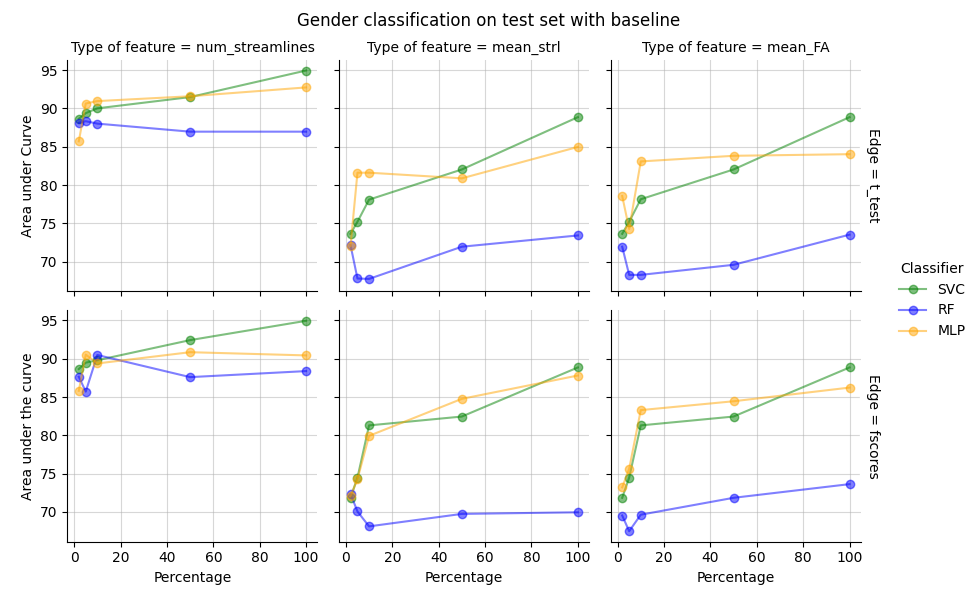
\includegraphics[width=\textwidth]{images/baseline_results_gender.png}
    \caption{Caption}
    \label{fig:my_label}
\end{figure}
\subsection{Solver based analysis}
Solver outputs 
\begin{figure}
    \centering
    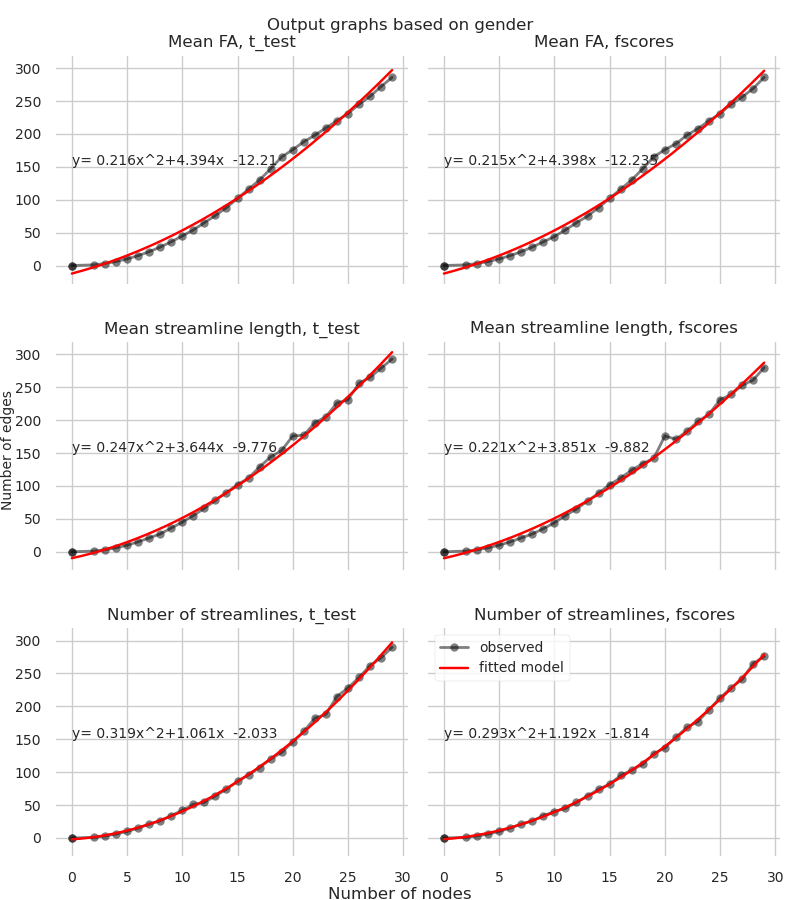
\includegraphics[width=0.8\textwidth]{images/Gender_nodes_preserved.png}
    \caption{Caption}
    \label{fig:my_label}
\end{figure}
\begin{figure}
    \centering
    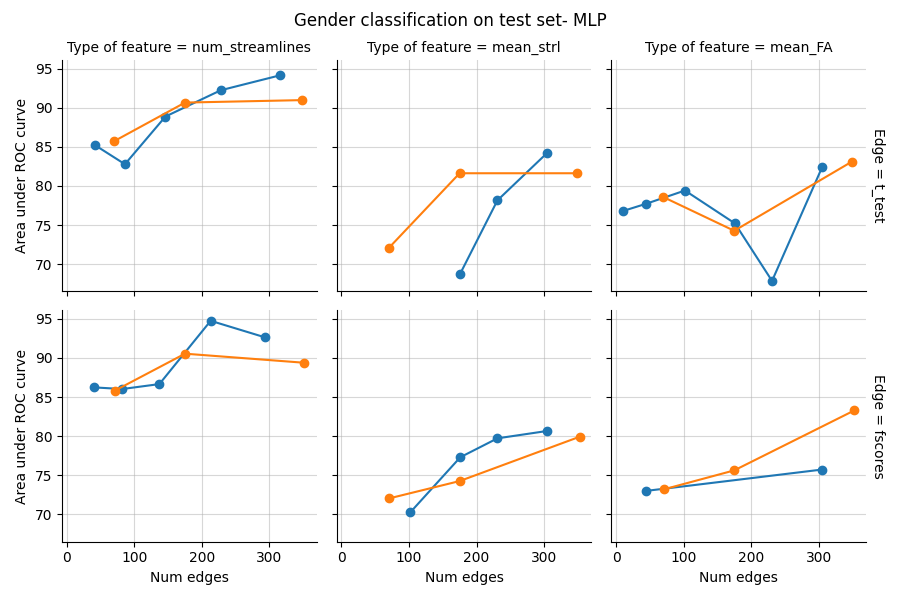
\includegraphics[width = \textwidth]{images/Gender_classification_comparison_MLP.png}
    \caption{Caption}
    \label{fig:my_label}
\end{figure}
\begin{figure}
    \centering
    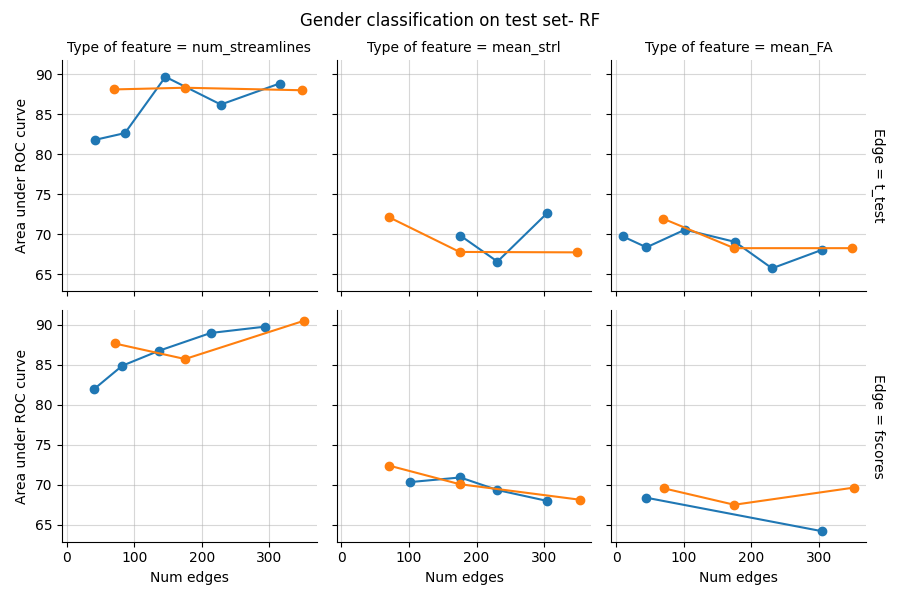
\includegraphics[width = \textwidth]{images/Gender_classification_comparison_RF.png}
    \caption{Caption}
    \label{fig:my_label}
\end{figure}

\subsection{Solver and baseline comparison}
\begin{figure}
    \centering
    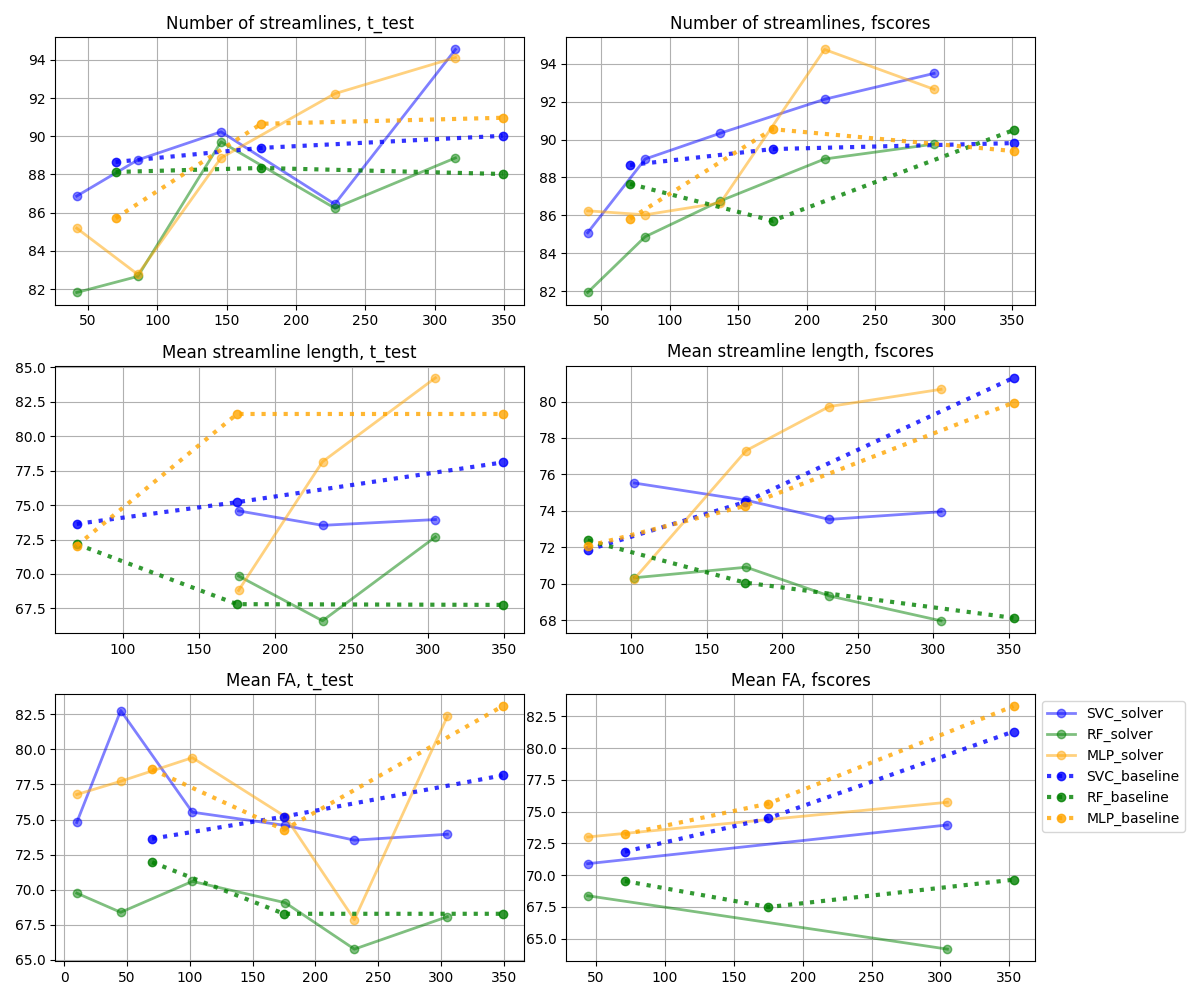
\includegraphics[width=\textwidth]{images/classification_gender_clf_combined.png}
    \caption{Caption}
    \label{fig:my_label}
\end{figure}
\begin{figure}
    \centering
    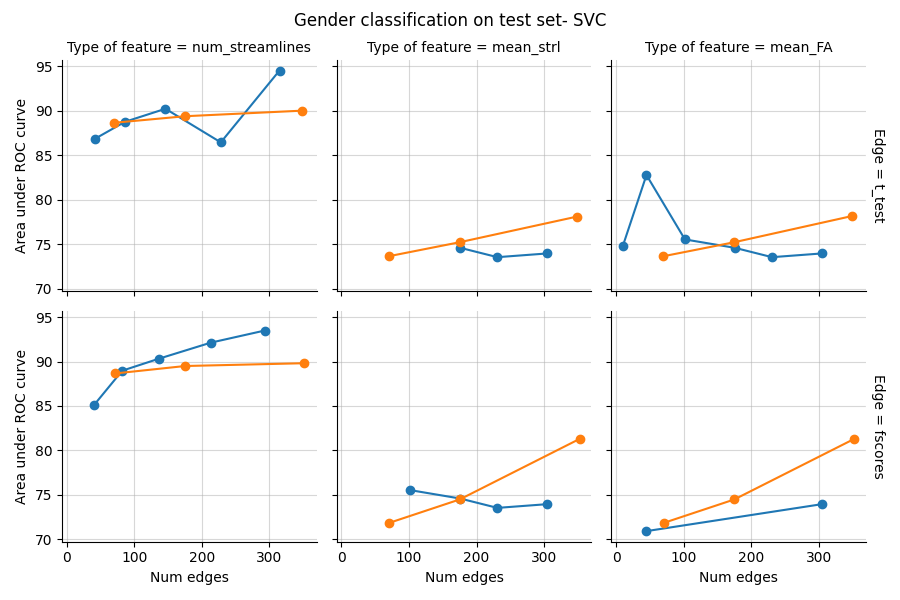
\includegraphics[width = \textwidth]{images/Gender_classification_comparison_SVC.png}
    \caption{Caption}
    \label{fig:my_label}
\end{figure}
\section{Interpretabilitiy}

\end{document}
